% Created by tikzDevice version 0.6.2-92-0ad2792 on 2013-03-03 12:19:45
% !TEX encoding = UTF-8 Unicode
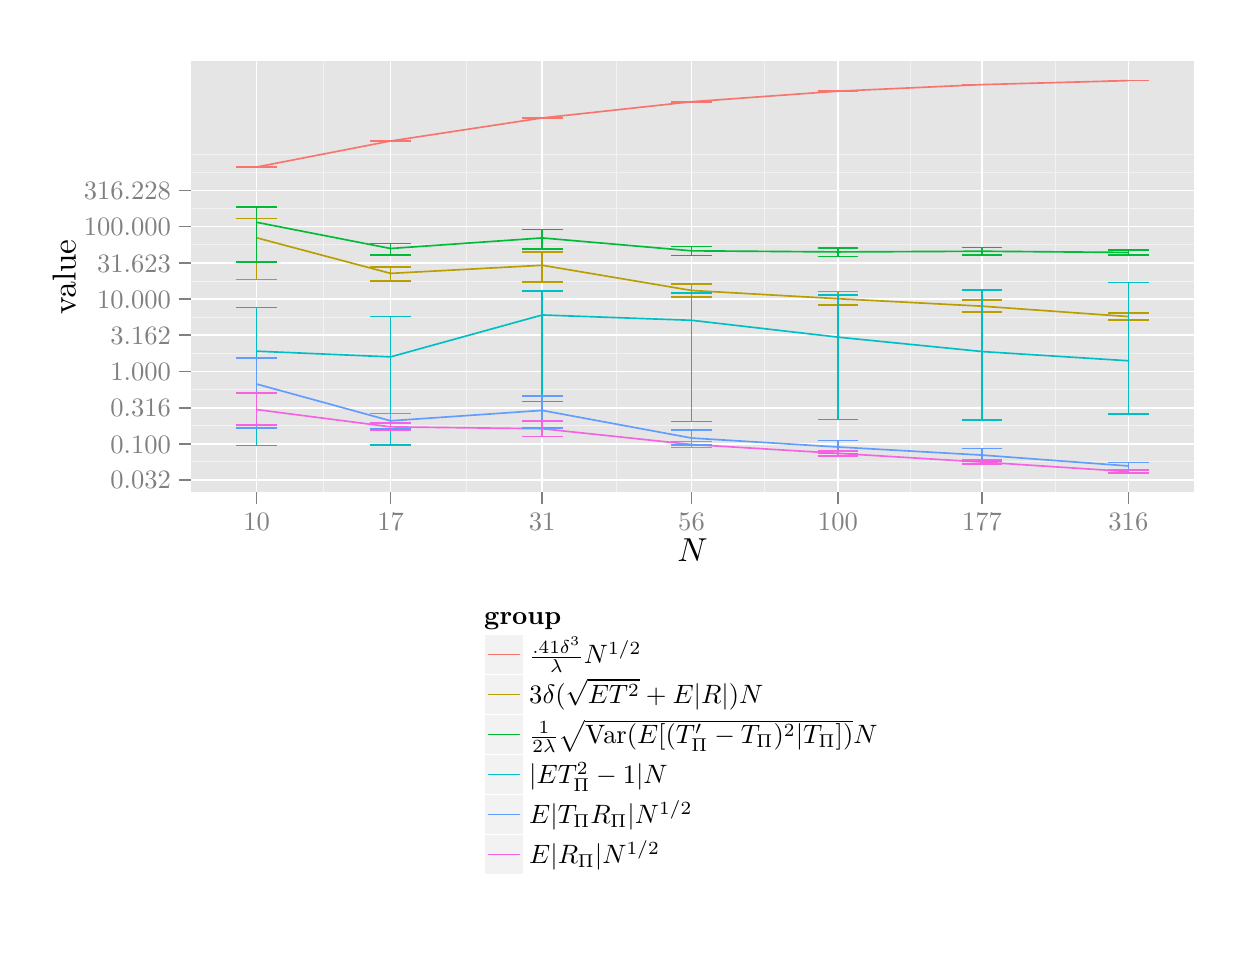
\begin{tikzpicture}[x=1pt,y=1pt]
\definecolor[named]{fillColor}{rgb}{1.00,1.00,1.00}
\path[use as bounding box,fill=fillColor,fill opacity=0.00] (0,0) rectangle (433.62,325.21);
\begin{scope}
\path[clip] (  0.00,  0.00) rectangle (433.62,325.21);
\definecolor[named]{drawColor}{rgb}{1.00,1.00,1.00}
\definecolor[named]{fillColor}{rgb}{1.00,1.00,1.00}

\path[draw=drawColor,line width= 0.6pt,line join=round,line cap=round,fill=fillColor] (  0.00,  0.00) rectangle (433.62,325.21);
\end{scope}
\begin{scope}
\path[clip] ( 58.88,157.27) rectangle (421.57,313.17);
\definecolor[named]{fillColor}{rgb}{0.90,0.90,0.90}

\path[fill=fillColor] ( 58.88,157.27) rectangle (421.57,313.17);
\definecolor[named]{drawColor}{rgb}{0.95,0.95,0.95}

\path[draw=drawColor,line width= 0.3pt,line join=round] ( 58.88,168.30) --
	(421.57,168.30);

\path[draw=drawColor,line width= 0.3pt,line join=round] ( 58.88,181.32) --
	(421.57,181.32);

\path[draw=drawColor,line width= 0.3pt,line join=round] ( 58.88,194.41) --
	(421.57,194.41);

\path[draw=drawColor,line width= 0.3pt,line join=round] ( 58.88,207.50) --
	(421.57,207.50);

\path[draw=drawColor,line width= 0.3pt,line join=round] ( 58.88,220.59) --
	(421.57,220.59);

\path[draw=drawColor,line width= 0.3pt,line join=round] ( 58.88,233.68) --
	(421.57,233.68);

\path[draw=drawColor,line width= 0.3pt,line join=round] ( 58.88,246.77) --
	(421.57,246.77);

\path[draw=drawColor,line width= 0.3pt,line join=round] ( 58.88,259.86) --
	(421.57,259.86);

\path[draw=drawColor,line width= 0.3pt,line join=round] ( 58.88,272.88) --
	(421.57,272.88);

\path[draw=drawColor,line width= 0.3pt,line join=round] ( 58.88,279.35) --
	(421.57,279.35);

\path[draw=drawColor,line width= 0.3pt,line join=round] (106.92,157.27) --
	(106.92,313.17);

\path[draw=drawColor,line width= 0.3pt,line join=round] (158.53,157.27) --
	(158.53,313.17);

\path[draw=drawColor,line width= 0.3pt,line join=round] (212.91,157.27) --
	(212.91,313.17);

\path[draw=drawColor,line width= 0.3pt,line join=round] (266.33,157.27) --
	(266.33,313.17);

\path[draw=drawColor,line width= 0.3pt,line join=round] (318.82,157.27) --
	(318.82,313.17);

\path[draw=drawColor,line width= 0.3pt,line join=round] (371.30,157.27) --
	(371.30,313.17);
\definecolor[named]{drawColor}{rgb}{1.00,1.00,1.00}

\path[draw=drawColor,line width= 0.6pt,line join=round] ( 58.88,161.82) --
	(421.57,161.82);

\path[draw=drawColor,line width= 0.6pt,line join=round] ( 58.88,174.78) --
	(421.57,174.78);

\path[draw=drawColor,line width= 0.6pt,line join=round] ( 58.88,187.86) --
	(421.57,187.86);

\path[draw=drawColor,line width= 0.6pt,line join=round] ( 58.88,200.95) --
	(421.57,200.95);

\path[draw=drawColor,line width= 0.6pt,line join=round] ( 58.88,214.04) --
	(421.57,214.04);

\path[draw=drawColor,line width= 0.6pt,line join=round] ( 58.88,227.13) --
	(421.57,227.13);

\path[draw=drawColor,line width= 0.6pt,line join=round] ( 58.88,240.22) --
	(421.57,240.22);

\path[draw=drawColor,line width= 0.6pt,line join=round] ( 58.88,253.31) --
	(421.57,253.31);

\path[draw=drawColor,line width= 0.6pt,line join=round] ( 58.88,266.40) --
	(421.57,266.40);

\path[draw=drawColor,line width= 0.6pt,line join=round] ( 82.72,157.27) --
	( 82.72,313.17);

\path[draw=drawColor,line width= 0.6pt,line join=round] (131.13,157.27) --
	(131.13,313.17);

\path[draw=drawColor,line width= 0.6pt,line join=round] (185.93,157.27) --
	(185.93,313.17);

\path[draw=drawColor,line width= 0.6pt,line join=round] (239.88,157.27) --
	(239.88,313.17);

\path[draw=drawColor,line width= 0.6pt,line join=round] (292.78,157.27) --
	(292.78,313.17);

\path[draw=drawColor,line width= 0.6pt,line join=round] (344.86,157.27) --
	(344.86,313.17);

\path[draw=drawColor,line width= 0.6pt,line join=round] (397.74,157.27) --
	(397.74,313.17);
\definecolor[named]{drawColor}{rgb}{0.97,0.46,0.43}

\path[draw=drawColor,line width= 0.6pt,line join=round] ( 82.72,274.85) --
	(131.13,284.25) --
	(185.93,292.59) --
	(239.88,298.44) --
	(292.78,302.26) --
	(344.86,304.63) --
	(397.74,306.08);
\definecolor[named]{drawColor}{rgb}{0.72,0.62,0.00}

\path[draw=drawColor,line width= 0.6pt,line join=round] ( 82.72,249.28) --
	(131.13,236.42) --
	(185.93,239.35) --
	(239.88,230.25) --
	(292.78,227.27) --
	(344.86,224.57) --
	(397.74,220.81);
\definecolor[named]{drawColor}{rgb}{0.00,0.73,0.22}

\path[draw=drawColor,line width= 0.6pt,line join=round] ( 82.72,254.88) --
	(131.13,245.41) --
	(185.93,249.23) --
	(239.88,244.57) --
	(292.78,244.17) --
	(344.86,244.42) --
	(397.74,243.98);
\definecolor[named]{drawColor}{rgb}{0.00,0.75,0.77}

\path[draw=drawColor,line width= 0.6pt,line join=round] ( 82.72,208.31) --
	(131.13,206.25) --
	(185.93,221.39) --
	(239.88,219.47) --
	(292.78,213.38) --
	(344.86,208.18) --
	(397.74,204.84);
\definecolor[named]{drawColor}{rgb}{0.38,0.61,1.00}

\path[draw=drawColor,line width= 0.6pt,line join=round] ( 82.72,196.43) --
	(131.13,183.15) --
	(185.93,186.91) --
	(239.88,176.92) --
	(292.78,173.69) --
	(344.86,170.76) --
	(397.74,166.83);
\definecolor[named]{drawColor}{rgb}{0.96,0.39,0.89}

\path[draw=drawColor,line width= 0.6pt,line join=round] ( 82.72,187.21) --
	(131.13,180.96) --
	(185.93,180.29) --
	(239.88,174.59) --
	(292.78,171.40) --
	(344.86,168.24) --
	(397.74,164.80);
\definecolor[named]{drawColor}{rgb}{0.97,0.46,0.43}

\path[draw=drawColor,line width= 0.6pt,line join=round] ( 75.37,274.85) --
	( 90.07,274.85);

\path[draw=drawColor,line width= 0.6pt,line join=round] ( 82.72,274.85) --
	( 82.72,274.85);

\path[draw=drawColor,line width= 0.6pt,line join=round] ( 75.37,274.85) --
	( 90.07,274.85);

\path[draw=drawColor,line width= 0.6pt,line join=round] (123.78,284.25) --
	(138.48,284.25);

\path[draw=drawColor,line width= 0.6pt,line join=round] (131.13,284.25) --
	(131.13,284.25);

\path[draw=drawColor,line width= 0.6pt,line join=round] (123.78,284.25) --
	(138.48,284.25);

\path[draw=drawColor,line width= 0.6pt,line join=round] (178.58,292.59) --
	(193.28,292.59);

\path[draw=drawColor,line width= 0.6pt,line join=round] (185.93,292.59) --
	(185.93,292.59);

\path[draw=drawColor,line width= 0.6pt,line join=round] (178.58,292.59) --
	(193.28,292.59);

\path[draw=drawColor,line width= 0.6pt,line join=round] (232.53,298.44) --
	(247.23,298.44);

\path[draw=drawColor,line width= 0.6pt,line join=round] (239.88,298.44) --
	(239.88,298.44);

\path[draw=drawColor,line width= 0.6pt,line join=round] (232.53,298.44) --
	(247.23,298.44);

\path[draw=drawColor,line width= 0.6pt,line join=round] (285.42,302.26) --
	(300.13,302.26);

\path[draw=drawColor,line width= 0.6pt,line join=round] (292.78,302.26) --
	(292.78,302.26);

\path[draw=drawColor,line width= 0.6pt,line join=round] (285.42,302.26) --
	(300.13,302.26);

\path[draw=drawColor,line width= 0.6pt,line join=round] (337.51,304.63) --
	(352.22,304.63);

\path[draw=drawColor,line width= 0.6pt,line join=round] (344.86,304.63) --
	(344.86,304.63);

\path[draw=drawColor,line width= 0.6pt,line join=round] (337.51,304.63) --
	(352.22,304.63);

\path[draw=drawColor,line width= 0.6pt,line join=round] (390.39,306.08) --
	(405.09,306.08);

\path[draw=drawColor,line width= 0.6pt,line join=round] (397.74,306.08) --
	(397.74,306.08);

\path[draw=drawColor,line width= 0.6pt,line join=round] (390.39,306.08) --
	(405.09,306.08);
\definecolor[named]{drawColor}{rgb}{0.72,0.62,0.00}

\path[draw=drawColor,line width= 0.6pt,line join=round] ( 75.37,256.20) --
	( 90.07,256.20);

\path[draw=drawColor,line width= 0.6pt,line join=round] ( 82.72,256.20) --
	( 82.72,234.20);

\path[draw=drawColor,line width= 0.6pt,line join=round] ( 75.37,234.20) --
	( 90.07,234.20);

\path[draw=drawColor,line width= 0.6pt,line join=round] (123.78,238.70) --
	(138.48,238.70);

\path[draw=drawColor,line width= 0.6pt,line join=round] (131.13,238.70) --
	(131.13,233.62);

\path[draw=drawColor,line width= 0.6pt,line join=round] (123.78,233.62) --
	(138.48,233.62);

\path[draw=drawColor,line width= 0.6pt,line join=round] (178.58,244.09) --
	(193.28,244.09);

\path[draw=drawColor,line width= 0.6pt,line join=round] (185.93,244.09) --
	(185.93,233.31);

\path[draw=drawColor,line width= 0.6pt,line join=round] (178.58,233.31) --
	(193.28,233.31);

\path[draw=drawColor,line width= 0.6pt,line join=round] (232.53,232.52) --
	(247.23,232.52);

\path[draw=drawColor,line width= 0.6pt,line join=round] (239.88,232.52) --
	(239.88,227.87);

\path[draw=drawColor,line width= 0.6pt,line join=round] (232.53,227.87) --
	(247.23,227.87);

\path[draw=drawColor,line width= 0.6pt,line join=round] (285.42,229.85) --
	(300.13,229.85);

\path[draw=drawColor,line width= 0.6pt,line join=round] (292.78,229.85) --
	(292.78,224.90);

\path[draw=drawColor,line width= 0.6pt,line join=round] (285.42,224.90) --
	(300.13,224.90);

\path[draw=drawColor,line width= 0.6pt,line join=round] (337.51,226.70) --
	(352.22,226.70);

\path[draw=drawColor,line width= 0.6pt,line join=round] (344.86,226.70) --
	(344.86,222.45);

\path[draw=drawColor,line width= 0.6pt,line join=round] (337.51,222.45) --
	(352.22,222.45);

\path[draw=drawColor,line width= 0.6pt,line join=round] (390.39,222.15) --
	(405.09,222.15);

\path[draw=drawColor,line width= 0.6pt,line join=round] (397.74,222.15) --
	(397.74,219.69);

\path[draw=drawColor,line width= 0.6pt,line join=round] (390.39,219.69) --
	(405.09,219.69);
\definecolor[named]{drawColor}{rgb}{0.00,0.73,0.22}

\path[draw=drawColor,line width= 0.6pt,line join=round] ( 75.37,260.31) --
	( 90.07,260.31);

\path[draw=drawColor,line width= 0.6pt,line join=round] ( 82.72,260.31) --
	( 82.72,240.51);

\path[draw=drawColor,line width= 0.6pt,line join=round] ( 75.37,240.51) --
	( 90.07,240.51);

\path[draw=drawColor,line width= 0.6pt,line join=round] (123.78,247.16) --
	(138.48,247.16);

\path[draw=drawColor,line width= 0.6pt,line join=round] (131.13,247.16) --
	(131.13,242.98);

\path[draw=drawColor,line width= 0.6pt,line join=round] (123.78,242.98) --
	(138.48,242.98);

\path[draw=drawColor,line width= 0.6pt,line join=round] (178.58,252.33) --
	(193.28,252.33);

\path[draw=drawColor,line width= 0.6pt,line join=round] (185.93,252.33) --
	(185.93,245.21);

\path[draw=drawColor,line width= 0.6pt,line join=round] (178.58,245.21) --
	(193.28,245.21);

\path[draw=drawColor,line width= 0.6pt,line join=round] (232.53,246.11) --
	(247.23,246.11);

\path[draw=drawColor,line width= 0.6pt,line join=round] (239.88,246.11) --
	(239.88,242.90);

\path[draw=drawColor,line width= 0.6pt,line join=round] (232.53,242.90) --
	(247.23,242.90);

\path[draw=drawColor,line width= 0.6pt,line join=round] (285.42,245.58) --
	(300.13,245.58);

\path[draw=drawColor,line width= 0.6pt,line join=round] (292.78,245.58) --
	(292.78,242.51);

\path[draw=drawColor,line width= 0.6pt,line join=round] (285.42,242.51) --
	(300.13,242.51);

\path[draw=drawColor,line width= 0.6pt,line join=round] (337.51,245.72) --
	(352.22,245.72);

\path[draw=drawColor,line width= 0.6pt,line join=round] (344.86,245.72) --
	(344.86,243.14);

\path[draw=drawColor,line width= 0.6pt,line join=round] (337.51,243.14) --
	(352.22,243.14);

\path[draw=drawColor,line width= 0.6pt,line join=round] (390.39,244.75) --
	(405.09,244.75);

\path[draw=drawColor,line width= 0.6pt,line join=round] (397.74,244.75) --
	(397.74,243.14);

\path[draw=drawColor,line width= 0.6pt,line join=round] (390.39,243.14) --
	(405.09,243.14);
\definecolor[named]{drawColor}{rgb}{0.00,0.75,0.77}

\path[draw=drawColor,line width= 0.6pt,line join=round] ( 75.37,224.14) --
	( 90.07,224.14);

\path[draw=drawColor,line width= 0.6pt,line join=round] ( 82.72,224.14) --
	( 82.72,174.17);

\path[draw=drawColor,line width= 0.6pt,line join=round] ( 75.37,174.17) --
	( 90.07,174.17);

\path[draw=drawColor,line width= 0.6pt,line join=round] (123.78,220.82) --
	(138.48,220.82);

\path[draw=drawColor,line width= 0.6pt,line join=round] (131.13,220.82) --
	(131.13,174.46);

\path[draw=drawColor,line width= 0.6pt,line join=round] (123.78,174.46) --
	(138.48,174.46);

\path[draw=drawColor,line width= 0.6pt,line join=round] (178.58,230.08) --
	(193.28,230.08);

\path[draw=drawColor,line width= 0.6pt,line join=round] (185.93,230.08) --
	(185.93,190.15);

\path[draw=drawColor,line width= 0.6pt,line join=round] (178.58,190.15) --
	(193.28,190.15);

\path[draw=drawColor,line width= 0.6pt,line join=round] (232.53,229.34) --
	(247.23,229.34);

\path[draw=drawColor,line width= 0.6pt,line join=round] (239.88,229.34) --
	(239.88,182.92);

\path[draw=drawColor,line width= 0.6pt,line join=round] (232.53,182.92) --
	(247.23,182.92);

\path[draw=drawColor,line width= 0.6pt,line join=round] (285.42,228.66) --
	(300.13,228.66);

\path[draw=drawColor,line width= 0.6pt,line join=round] (292.78,228.66) --
	(292.78,183.66);

\path[draw=drawColor,line width= 0.6pt,line join=round] (285.42,183.66) --
	(300.13,183.66);

\path[draw=drawColor,line width= 0.6pt,line join=round] (337.51,230.44) --
	(352.22,230.44);

\path[draw=drawColor,line width= 0.6pt,line join=round] (344.86,230.44) --
	(344.86,183.51);

\path[draw=drawColor,line width= 0.6pt,line join=round] (337.51,183.51) --
	(352.22,183.51);

\path[draw=drawColor,line width= 0.6pt,line join=round] (390.39,233.18) --
	(405.09,233.18);

\path[draw=drawColor,line width= 0.6pt,line join=round] (397.74,233.18) --
	(397.74,185.71);

\path[draw=drawColor,line width= 0.6pt,line join=round] (390.39,185.71) --
	(405.09,185.71);
\definecolor[named]{drawColor}{rgb}{0.38,0.61,1.00}

\path[draw=drawColor,line width= 0.6pt,line join=round] ( 75.37,205.89) --
	( 90.07,205.89);

\path[draw=drawColor,line width= 0.6pt,line join=round] ( 82.72,205.89) --
	( 82.72,180.58);

\path[draw=drawColor,line width= 0.6pt,line join=round] ( 75.37,180.58) --
	( 90.07,180.58);

\path[draw=drawColor,line width= 0.6pt,line join=round] (123.78,185.85) --
	(138.48,185.85);

\path[draw=drawColor,line width= 0.6pt,line join=round] (131.13,185.85) --
	(131.13,180.07);

\path[draw=drawColor,line width= 0.6pt,line join=round] (123.78,180.07) --
	(138.48,180.07);

\path[draw=drawColor,line width= 0.6pt,line join=round] (178.58,192.17) --
	(193.28,192.17);

\path[draw=drawColor,line width= 0.6pt,line join=round] (185.93,192.17) --
	(185.93,180.52);

\path[draw=drawColor,line width= 0.6pt,line join=round] (178.58,180.52) --
	(193.28,180.52);

\path[draw=drawColor,line width= 0.6pt,line join=round] (232.53,179.84) --
	(247.23,179.84);

\path[draw=drawColor,line width= 0.6pt,line join=round] (239.88,179.84) --
	(239.88,174.32);

\path[draw=drawColor,line width= 0.6pt,line join=round] (232.53,174.32) --
	(247.23,174.32);

\path[draw=drawColor,line width= 0.6pt,line join=round] (285.42,175.99) --
	(300.13,175.99);

\path[draw=drawColor,line width= 0.6pt,line join=round] (292.78,175.99) --
	(292.78,171.30);

\path[draw=drawColor,line width= 0.6pt,line join=round] (285.42,171.30) --
	(300.13,171.30);

\path[draw=drawColor,line width= 0.6pt,line join=round] (337.51,173.17) --
	(352.22,173.17);

\path[draw=drawColor,line width= 0.6pt,line join=round] (344.86,173.17) --
	(344.86,168.46);

\path[draw=drawColor,line width= 0.6pt,line join=round] (337.51,168.46) --
	(352.22,168.46);

\path[draw=drawColor,line width= 0.6pt,line join=round] (390.39,168.12) --
	(405.09,168.12);

\path[draw=drawColor,line width= 0.6pt,line join=round] (397.74,168.12) --
	(397.74,165.56);

\path[draw=drawColor,line width= 0.6pt,line join=round] (390.39,165.56) --
	(405.09,165.56);
\definecolor[named]{drawColor}{rgb}{0.96,0.39,0.89}

\path[draw=drawColor,line width= 0.6pt,line join=round] ( 75.37,193.29) --
	( 90.07,193.29);

\path[draw=drawColor,line width= 0.6pt,line join=round] ( 82.72,193.29) --
	( 82.72,181.65);

\path[draw=drawColor,line width= 0.6pt,line join=round] ( 75.37,181.65) --
	( 90.07,181.65);

\path[draw=drawColor,line width= 0.6pt,line join=round] (123.78,182.30) --
	(138.48,182.30);

\path[draw=drawColor,line width= 0.6pt,line join=round] (131.13,182.30) --
	(131.13,179.62);

\path[draw=drawColor,line width= 0.6pt,line join=round] (123.78,179.62) --
	(138.48,179.62);

\path[draw=drawColor,line width= 0.6pt,line join=round] (178.58,183.02) --
	(193.28,183.02);

\path[draw=drawColor,line width= 0.6pt,line join=round] (185.93,183.02) --
	(185.93,177.45);

\path[draw=drawColor,line width= 0.6pt,line join=round] (178.58,177.45) --
	(193.28,177.45);

\path[draw=drawColor,line width= 0.6pt,line join=round] (232.53,175.66) --
	(247.23,175.66);

\path[draw=drawColor,line width= 0.6pt,line join=round] (239.88,175.66) --
	(239.88,173.47);

\path[draw=drawColor,line width= 0.6pt,line join=round] (232.53,173.47) --
	(247.23,173.47);

\path[draw=drawColor,line width= 0.6pt,line join=round] (285.42,172.34) --
	(300.13,172.34);

\path[draw=drawColor,line width= 0.6pt,line join=round] (292.78,172.34) --
	(292.78,170.54);

\path[draw=drawColor,line width= 0.6pt,line join=round] (285.42,170.54) --
	(300.13,170.54);

\path[draw=drawColor,line width= 0.6pt,line join=round] (337.51,169.10) --
	(352.22,169.10);

\path[draw=drawColor,line width= 0.6pt,line join=round] (344.86,169.10) --
	(344.86,167.53);

\path[draw=drawColor,line width= 0.6pt,line join=round] (337.51,167.53) --
	(352.22,167.53);

\path[draw=drawColor,line width= 0.6pt,line join=round] (390.39,165.29) --
	(405.09,165.29);

\path[draw=drawColor,line width= 0.6pt,line join=round] (397.74,165.29) --
	(397.74,164.35);

\path[draw=drawColor,line width= 0.6pt,line join=round] (390.39,164.35) --
	(405.09,164.35);
\end{scope}
\begin{scope}
\path[clip] (  0.00,  0.00) rectangle (433.62,325.21);
\definecolor[named]{drawColor}{rgb}{0.50,0.50,0.50}

\node[text=drawColor,anchor=base east,inner sep=0pt, outer sep=0pt, scale=  0.96] at ( 51.77,158.52) {0.032};

\node[text=drawColor,anchor=base east,inner sep=0pt, outer sep=0pt, scale=  0.96] at ( 51.77,171.47) {0.100};

\node[text=drawColor,anchor=base east,inner sep=0pt, outer sep=0pt, scale=  0.96] at ( 51.77,184.55) {0.316};

\node[text=drawColor,anchor=base east,inner sep=0pt, outer sep=0pt, scale=  0.96] at ( 51.77,197.65) {1.000};

\node[text=drawColor,anchor=base east,inner sep=0pt, outer sep=0pt, scale=  0.96] at ( 51.77,210.74) {3.162};

\node[text=drawColor,anchor=base east,inner sep=0pt, outer sep=0pt, scale=  0.96] at ( 51.77,223.83) {10.000};

\node[text=drawColor,anchor=base east,inner sep=0pt, outer sep=0pt, scale=  0.96] at ( 51.77,236.92) {31.623};

\node[text=drawColor,anchor=base east,inner sep=0pt, outer sep=0pt, scale=  0.96] at ( 51.77,250.01) {100.000};

\node[text=drawColor,anchor=base east,inner sep=0pt, outer sep=0pt, scale=  0.96] at ( 51.77,263.09) {316.228};
\end{scope}
\begin{scope}
\path[clip] (  0.00,  0.00) rectangle (433.62,325.21);
\definecolor[named]{drawColor}{rgb}{0.50,0.50,0.50}

\path[draw=drawColor,line width= 0.6pt,line join=round] ( 54.61,161.82) --
	( 58.88,161.82);

\path[draw=drawColor,line width= 0.6pt,line join=round] ( 54.61,174.78) --
	( 58.88,174.78);

\path[draw=drawColor,line width= 0.6pt,line join=round] ( 54.61,187.86) --
	( 58.88,187.86);

\path[draw=drawColor,line width= 0.6pt,line join=round] ( 54.61,200.95) --
	( 58.88,200.95);

\path[draw=drawColor,line width= 0.6pt,line join=round] ( 54.61,214.04) --
	( 58.88,214.04);

\path[draw=drawColor,line width= 0.6pt,line join=round] ( 54.61,227.13) --
	( 58.88,227.13);

\path[draw=drawColor,line width= 0.6pt,line join=round] ( 54.61,240.22) --
	( 58.88,240.22);

\path[draw=drawColor,line width= 0.6pt,line join=round] ( 54.61,253.31) --
	( 58.88,253.31);

\path[draw=drawColor,line width= 0.6pt,line join=round] ( 54.61,266.40) --
	( 58.88,266.40);
\end{scope}
\begin{scope}
\path[clip] (  0.00,  0.00) rectangle (433.62,325.21);
\definecolor[named]{drawColor}{rgb}{0.50,0.50,0.50}

\path[draw=drawColor,line width= 0.6pt,line join=round] ( 82.72,153.00) --
	( 82.72,157.27);

\path[draw=drawColor,line width= 0.6pt,line join=round] (131.13,153.00) --
	(131.13,157.27);

\path[draw=drawColor,line width= 0.6pt,line join=round] (185.93,153.00) --
	(185.93,157.27);

\path[draw=drawColor,line width= 0.6pt,line join=round] (239.88,153.00) --
	(239.88,157.27);

\path[draw=drawColor,line width= 0.6pt,line join=round] (292.78,153.00) --
	(292.78,157.27);

\path[draw=drawColor,line width= 0.6pt,line join=round] (344.86,153.00) --
	(344.86,157.27);

\path[draw=drawColor,line width= 0.6pt,line join=round] (397.74,153.00) --
	(397.74,157.27);
\end{scope}
\begin{scope}
\path[clip] (  0.00,  0.00) rectangle (433.62,325.21);
\definecolor[named]{drawColor}{rgb}{0.50,0.50,0.50}

\node[text=drawColor,anchor=base,inner sep=0pt, outer sep=0pt, scale=  0.96] at ( 82.72,143.54) {10};

\node[text=drawColor,anchor=base,inner sep=0pt, outer sep=0pt, scale=  0.96] at (131.13,143.54) {17};

\node[text=drawColor,anchor=base,inner sep=0pt, outer sep=0pt, scale=  0.96] at (185.93,143.54) {31};

\node[text=drawColor,anchor=base,inner sep=0pt, outer sep=0pt, scale=  0.96] at (239.88,143.54) {56};

\node[text=drawColor,anchor=base,inner sep=0pt, outer sep=0pt, scale=  0.96] at (292.78,143.54) {100};

\node[text=drawColor,anchor=base,inner sep=0pt, outer sep=0pt, scale=  0.96] at (344.86,143.54) {177};

\node[text=drawColor,anchor=base,inner sep=0pt, outer sep=0pt, scale=  0.96] at (397.74,143.54) {316};
\end{scope}
\begin{scope}
\path[clip] (  0.00,  0.00) rectangle (433.62,325.21);
\definecolor[named]{drawColor}{rgb}{0.00,0.00,0.00}

\node[text=drawColor,anchor=base,inner sep=0pt, outer sep=0pt, scale=  1.20] at (240.23,132.27) {$N$};
\end{scope}
\begin{scope}
\path[clip] (  0.00,  0.00) rectangle (433.62,325.21);
\definecolor[named]{drawColor}{rgb}{0.00,0.00,0.00}

\node[text=drawColor,rotate= 90.00,anchor=base,inner sep=0pt, outer sep=0pt, scale=  1.20] at ( 17.30,235.22) {value};
\end{scope}
\begin{scope}
\path[clip] (  0.00,  0.00) rectangle (433.62,325.21);
\definecolor[named]{fillColor}{rgb}{1.00,1.00,1.00}

\path[fill=fillColor] (160.71, 14.89) rectangle (319.75,120.39);
\end{scope}
\begin{scope}
\path[clip] (  0.00,  0.00) rectangle (433.62,325.21);
\definecolor[named]{drawColor}{rgb}{0.00,0.00,0.00}

\node[text=drawColor,anchor=base west,inner sep=0pt, outer sep=0pt, scale=  0.96] at (164.98,109.50) {\bfseries group};
\end{scope}
\begin{scope}
\path[clip] (  0.00,  0.00) rectangle (433.62,325.21);
\definecolor[named]{drawColor}{rgb}{1.00,1.00,1.00}
\definecolor[named]{fillColor}{rgb}{0.95,0.95,0.95}

\path[draw=drawColor,line width= 0.6pt,line join=round,line cap=round,fill=fillColor] (164.98, 91.43) rectangle (179.43,105.88);
\end{scope}
\begin{scope}
\path[clip] (  0.00,  0.00) rectangle (433.62,325.21);
\definecolor[named]{drawColor}{rgb}{0.97,0.46,0.43}

\path[draw=drawColor,line width= 0.6pt,line join=round] (166.42, 98.66) -- (177.98, 98.66);
\end{scope}
\begin{scope}
\path[clip] (  0.00,  0.00) rectangle (433.62,325.21);
\definecolor[named]{drawColor}{rgb}{0.97,0.46,0.43}

\path[draw=drawColor,line width= 0.6pt,line join=round] (166.42, 98.66) -- (177.98, 98.66);
\end{scope}
\begin{scope}
\path[clip] (  0.00,  0.00) rectangle (433.62,325.21);
\definecolor[named]{drawColor}{rgb}{1.00,1.00,1.00}
\definecolor[named]{fillColor}{rgb}{0.95,0.95,0.95}

\path[draw=drawColor,line width= 0.6pt,line join=round,line cap=round,fill=fillColor] (164.98, 76.97) rectangle (179.43, 91.43);
\end{scope}
\begin{scope}
\path[clip] (  0.00,  0.00) rectangle (433.62,325.21);
\definecolor[named]{drawColor}{rgb}{0.72,0.62,0.00}

\path[draw=drawColor,line width= 0.6pt,line join=round] (166.42, 84.20) -- (177.98, 84.20);
\end{scope}
\begin{scope}
\path[clip] (  0.00,  0.00) rectangle (433.62,325.21);
\definecolor[named]{drawColor}{rgb}{0.72,0.62,0.00}

\path[draw=drawColor,line width= 0.6pt,line join=round] (166.42, 84.20) -- (177.98, 84.20);
\end{scope}
\begin{scope}
\path[clip] (  0.00,  0.00) rectangle (433.62,325.21);
\definecolor[named]{drawColor}{rgb}{1.00,1.00,1.00}
\definecolor[named]{fillColor}{rgb}{0.95,0.95,0.95}

\path[draw=drawColor,line width= 0.6pt,line join=round,line cap=round,fill=fillColor] (164.98, 62.52) rectangle (179.43, 76.97);
\end{scope}
\begin{scope}
\path[clip] (  0.00,  0.00) rectangle (433.62,325.21);
\definecolor[named]{drawColor}{rgb}{0.00,0.73,0.22}

\path[draw=drawColor,line width= 0.6pt,line join=round] (166.42, 69.75) -- (177.98, 69.75);
\end{scope}
\begin{scope}
\path[clip] (  0.00,  0.00) rectangle (433.62,325.21);
\definecolor[named]{drawColor}{rgb}{0.00,0.73,0.22}

\path[draw=drawColor,line width= 0.6pt,line join=round] (166.42, 69.75) -- (177.98, 69.75);
\end{scope}
\begin{scope}
\path[clip] (  0.00,  0.00) rectangle (433.62,325.21);
\definecolor[named]{drawColor}{rgb}{1.00,1.00,1.00}
\definecolor[named]{fillColor}{rgb}{0.95,0.95,0.95}

\path[draw=drawColor,line width= 0.6pt,line join=round,line cap=round,fill=fillColor] (164.98, 48.07) rectangle (179.43, 62.52);
\end{scope}
\begin{scope}
\path[clip] (  0.00,  0.00) rectangle (433.62,325.21);
\definecolor[named]{drawColor}{rgb}{0.00,0.75,0.77}

\path[draw=drawColor,line width= 0.6pt,line join=round] (166.42, 55.29) -- (177.98, 55.29);
\end{scope}
\begin{scope}
\path[clip] (  0.00,  0.00) rectangle (433.62,325.21);
\definecolor[named]{drawColor}{rgb}{0.00,0.75,0.77}

\path[draw=drawColor,line width= 0.6pt,line join=round] (166.42, 55.29) -- (177.98, 55.29);
\end{scope}
\begin{scope}
\path[clip] (  0.00,  0.00) rectangle (433.62,325.21);
\definecolor[named]{drawColor}{rgb}{1.00,1.00,1.00}
\definecolor[named]{fillColor}{rgb}{0.95,0.95,0.95}

\path[draw=drawColor,line width= 0.6pt,line join=round,line cap=round,fill=fillColor] (164.98, 33.61) rectangle (179.43, 48.07);
\end{scope}
\begin{scope}
\path[clip] (  0.00,  0.00) rectangle (433.62,325.21);
\definecolor[named]{drawColor}{rgb}{0.38,0.61,1.00}

\path[draw=drawColor,line width= 0.6pt,line join=round] (166.42, 40.84) -- (177.98, 40.84);
\end{scope}
\begin{scope}
\path[clip] (  0.00,  0.00) rectangle (433.62,325.21);
\definecolor[named]{drawColor}{rgb}{0.38,0.61,1.00}

\path[draw=drawColor,line width= 0.6pt,line join=round] (166.42, 40.84) -- (177.98, 40.84);
\end{scope}
\begin{scope}
\path[clip] (  0.00,  0.00) rectangle (433.62,325.21);
\definecolor[named]{drawColor}{rgb}{1.00,1.00,1.00}
\definecolor[named]{fillColor}{rgb}{0.95,0.95,0.95}

\path[draw=drawColor,line width= 0.6pt,line join=round,line cap=round,fill=fillColor] (164.98, 19.16) rectangle (179.43, 33.61);
\end{scope}
\begin{scope}
\path[clip] (  0.00,  0.00) rectangle (433.62,325.21);
\definecolor[named]{drawColor}{rgb}{0.96,0.39,0.89}

\path[draw=drawColor,line width= 0.6pt,line join=round] (166.42, 26.39) -- (177.98, 26.39);
\end{scope}
\begin{scope}
\path[clip] (  0.00,  0.00) rectangle (433.62,325.21);
\definecolor[named]{drawColor}{rgb}{0.96,0.39,0.89}

\path[draw=drawColor,line width= 0.6pt,line join=round] (166.42, 26.39) -- (177.98, 26.39);
\end{scope}
\begin{scope}
\path[clip] (  0.00,  0.00) rectangle (433.62,325.21);
\definecolor[named]{drawColor}{rgb}{0.00,0.00,0.00}

\node[text=drawColor,anchor=base west,inner sep=0pt, outer sep=0pt, scale=  0.96] at (181.24, 95.35) {$\frac{.41\delta^3}{\lambda}N^{1/2}\quad $};
\end{scope}
\begin{scope}
\path[clip] (  0.00,  0.00) rectangle (433.62,325.21);
\definecolor[named]{drawColor}{rgb}{0.00,0.00,0.00}

\node[text=drawColor,anchor=base west,inner sep=0pt, outer sep=0pt, scale=  0.96] at (181.24, 80.90) {$3\delta(\sqrt{\mathbb{E}T^2}+\mathbb{E}|R|)N\quad $};
\end{scope}
\begin{scope}
\path[clip] (  0.00,  0.00) rectangle (433.62,325.21);
\definecolor[named]{drawColor}{rgb}{0.00,0.00,0.00}

\node[text=drawColor,anchor=base west,inner sep=0pt, outer sep=0pt, scale=  0.96] at (181.24, 66.44) {$\frac{1}{2\lambda}\sqrt{\mathrm{Var}(\mathbb{E}[(T'_{\Pi}-T_{\Pi})^2|T_{\Pi}])}N\quad $};
\end{scope}
\begin{scope}
\path[clip] (  0.00,  0.00) rectangle (433.62,325.21);
\definecolor[named]{drawColor}{rgb}{0.00,0.00,0.00}

\node[text=drawColor,anchor=base west,inner sep=0pt, outer sep=0pt, scale=  0.96] at (181.24, 51.99) {$|\mathbb{E}T_{\Pi}^2-1|N\quad $};
\end{scope}
\begin{scope}
\path[clip] (  0.00,  0.00) rectangle (433.62,325.21);
\definecolor[named]{drawColor}{rgb}{0.00,0.00,0.00}

\node[text=drawColor,anchor=base west,inner sep=0pt, outer sep=0pt, scale=  0.96] at (181.24, 37.53) {$\mathbb{E}|T_{\Pi}R_{\Pi}|N^{1/2}\quad $};
\end{scope}
\begin{scope}
\path[clip] (  0.00,  0.00) rectangle (433.62,325.21);
\definecolor[named]{drawColor}{rgb}{0.00,0.00,0.00}

\node[text=drawColor,anchor=base west,inner sep=0pt, outer sep=0pt, scale=  0.96] at (181.24, 23.08) {$\mathbb{E}|R_{\Pi}|N^{1/2}\quad $};
\end{scope}
\end{tikzpicture}
